

\section{Definitionen und Technologie}
\label{sec:definitionen-und-technologie}

TODOs:

\subsection{SAE-Level}
\label{ssec:sae-level}

Die SAE-Level \cite{standardSAE} beschreiben die Grad an Autonomie bei autonomen Fahrzeugen.\\

\textbf{Level 0 - Keine Automatisierung.} Der Fahrer übernimmt die volle Kontrolle über das Fahrzeug.

\textbf{Level 1 - Fahrassistenz.} Der Fahrer wird durch einen einzelnen Fahrassistenten, z.B. Tempomat, Spurhalteassistent oder Bremsassistent, unterstützt, behält jedoch die volle Kontrolle über das Fahrzeug.

\textbf{Level 2 - Partielle Automatisierung.} Der Fahrer wird durch mehrere Fahrassistenten unterstützt and hat immer die Kontrolle über das Fahrzeug.
    
\textbf{Level 3 - Bedingte Automatisierung.}
Das Fahrzeug ist in der Lage die Umgebung zu erkennen und ist in der Lage eigenständig in bestimmten Fahrsituationen zu meistern. Ein aufmerksamer Fahrer ist noch erforderlich, der unter Umständen einschreiten kann.

\textbf{Level 4 - Hohe Automatisierung.} Das Fahrzeug ist in der Lage sich eigenständig in den meisten Fahrumgebungen zu manövrieren. Es erkennt Fehlentscheidungen und kann auf diese reagieren. Menschliches einschreiten ist, wenn gewünscht, möglich.

\textbf{Level 5 - Volle Automatisierung.} Das Fahrzeug kann in allen Umgebungen und zu jederzeit und in jeder Situation komplett eigenständig Fahren.

\subsection{Sensoren}


\begin{figure}[H]
    \centering
    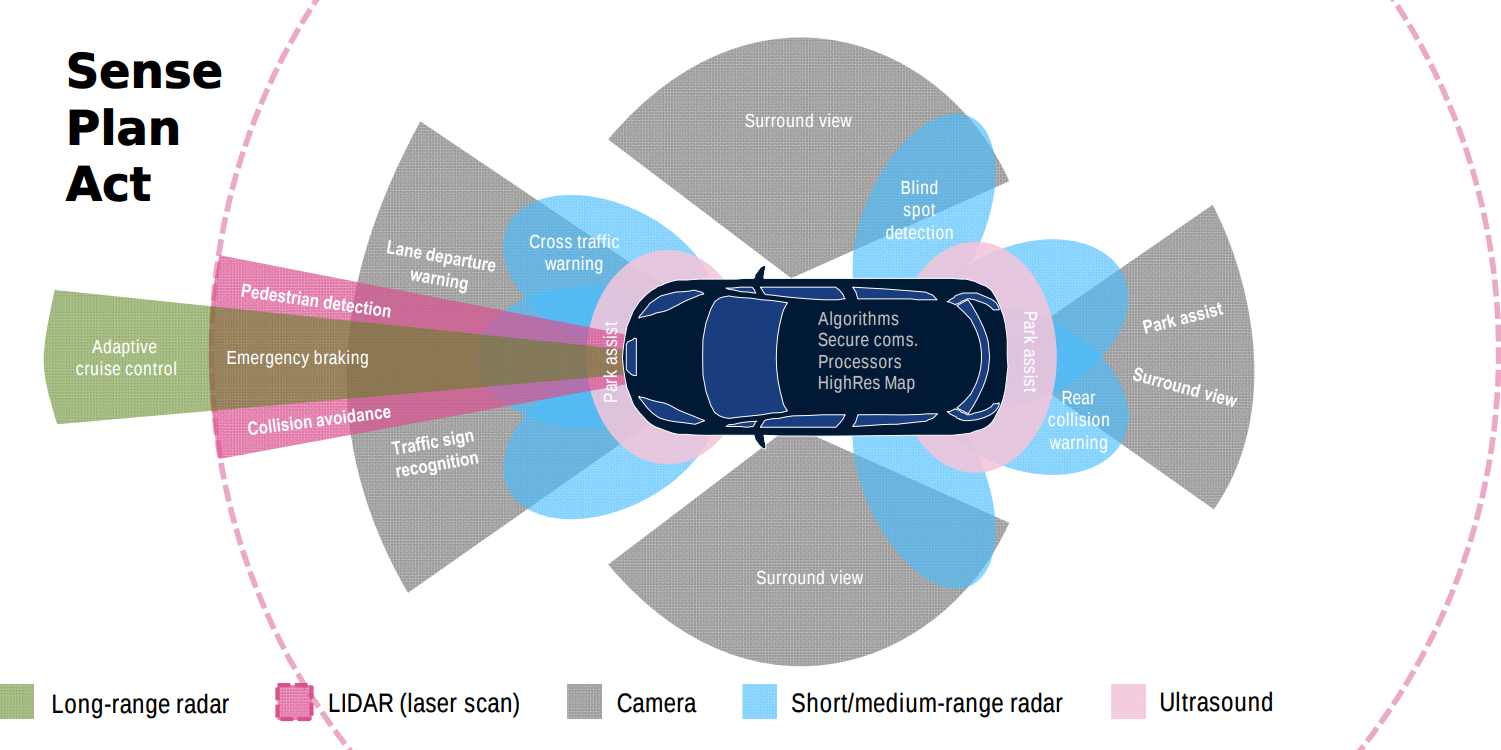
\includegraphics[width=.485\textwidth]{resources/images/sensors.png}
    \caption{Sensoren eines autonomen Fahrzeugs \cite{smith2015automated}}
\end{figure}



\subsection{Vehicular Ad-hoc Network}

\begin{figure}[H]
    \centering
    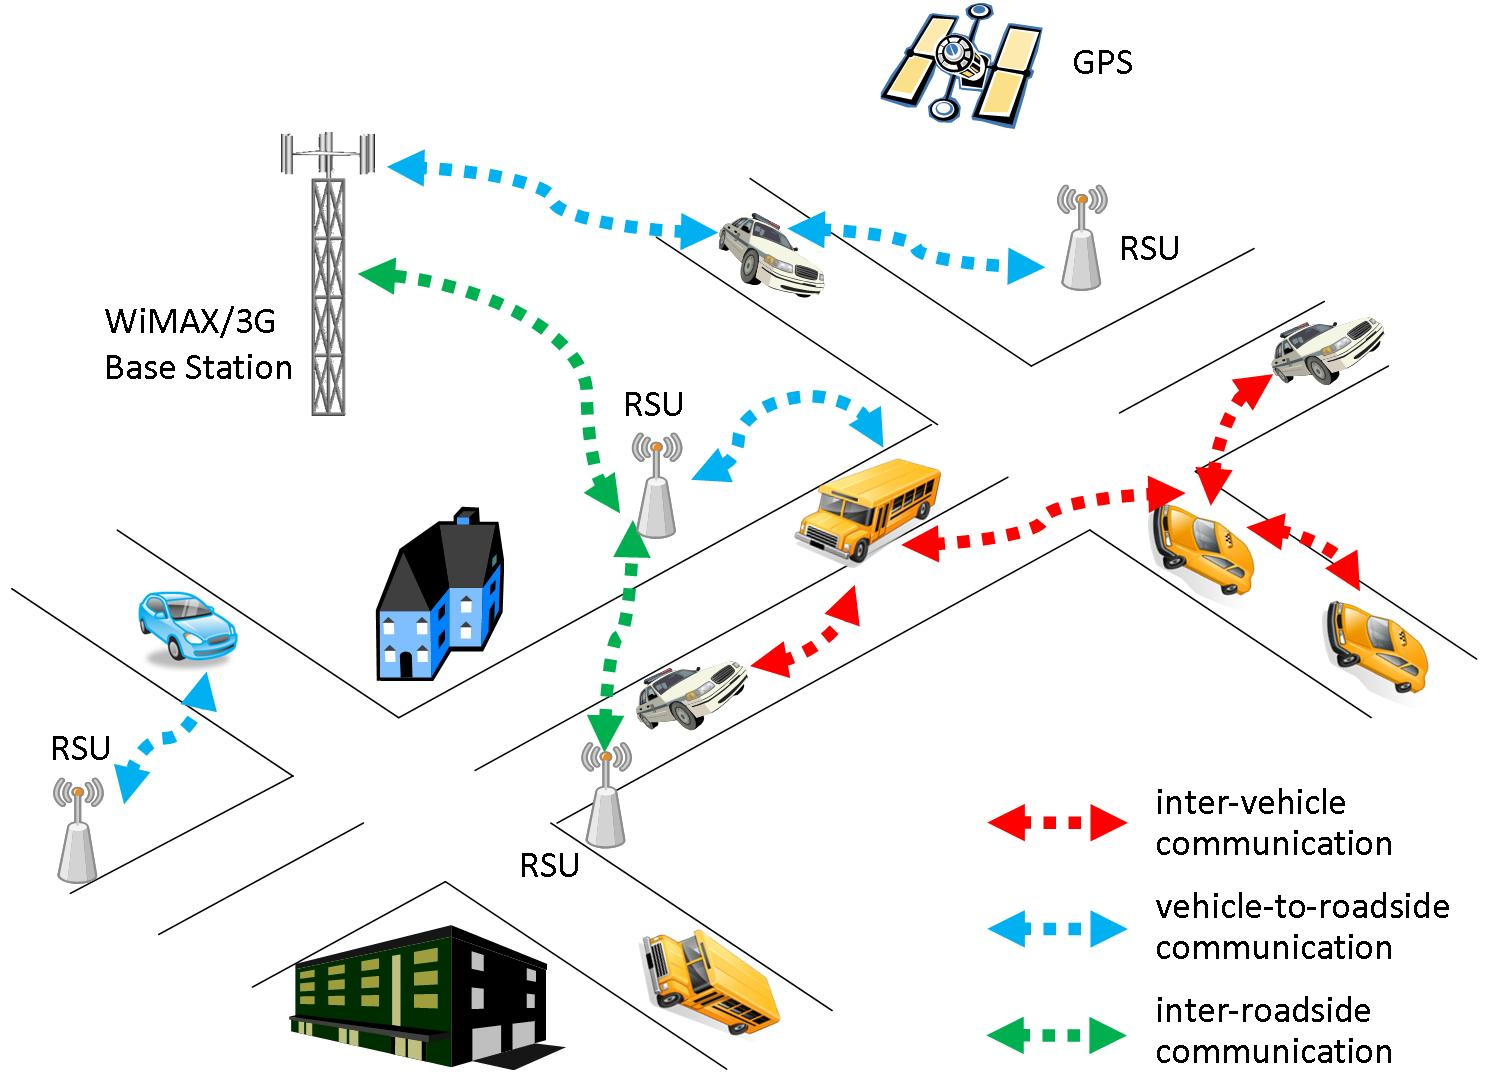
\includegraphics[width=.485\textwidth]{resources/images/vanet.jpg}
    \caption{Übersichtsgrafik eines VANETs \cite{vanet}}
\end{figure}

\subsection{Software}
TODO: